\section{Problem Description}

To motivate the problem of estimating thermal coupling between microzones, we provide a brief overview of buildings and their control systems.
Then, we discuss the potential utility of statistical models over complex physical building models, and how we apply parameter estimation in an Ising model to a particular building modeling problem.

\subsection{Motivation}

%As of 2012, 14\% of the buildings in the U.S. used building management systems (BMS) to manage and control the networked building infrastructure, usually consisting of lights, HVAC and electrical subsystems~\cite{cbecs2012}.

Occupant comfort is a major concern in building operation.
Standards bodies such as ASHRAE (the American Society of Heating, Refrigerating and Air-Conditioning Engineers) publish guidelines for how to maintain comfortable conditions within buildings~\cite{givoni1992comfort}.
Despite such standards, occupants are not actually comfortable; a 2006 survey of over 200 buildings across North America and Finland found that only 39\% of building occupants are satisfied with the temperature of their environment~\cite{huizenga2006air}.
This is an unfortunate number, especially when compared against ASHRAE's occupancy satisfaction goal of 80\%.
There are many factors that affect occupant comfort, but among the major factors is the inability of current building management systems to account for temperature gradients the spaces it conditions.

First, we present a brief overview of a canonical HVAC system which provides thermal conditioning for the space inside.
As seen in Figure~\ref{fig:example_building}, an Air Handling Unit (AHU) supplies air to a set of Variable Air Volume boxes (VAVs), which each supply air to a set of rooms (this set of rooms is known as an ``HVAC Zone'').
The air supplied by the AHU is typically cold -- usually between 55 and 65 degrees Fahrenheit -- so the damper in a VAV controls the strength of the airflow (and therefore the amount of cooling) for an HVAC zone.
The control loop in VAV modulates the damper to maintain the temperature of the room, which is given by the control loop's \emph{setpoint}: opening the damper more increases the flow of cold air into the room, which is measured by the thermostat, and the updated temperature is incorporated into the next ``tick'' of the control loop.

While simple to understand and implement, this basic arrangement of sensor inputs and control outputs (e.g. the damper position and temperature setpoint) makes the assumption that \emph{temperature is uniform across all spaces in an HVAC zone}.
This is trivially false; across rooms in an HVAC zone, differences in internal thermal load and inertia affect how much heat a physical space generates and retains.
Heat generation can come from the sun, people (a person is roughly the equivalent of a 100W light bulb), and appliances.
This generated heat is offset by windows, doors, fans and the HVAC system.
The end result is an HVAC zone that is ``comfortable'' only in the room where it measures temperature, and is either too cold or too warm in the other rooms.
To increase comfort, we want the building management system to make control decisions contingent on how heat diffuses through a set of rooms in an HVAC zone.

While it is possible to generate relatively accurate physical models of building spaces using software such as Modelica~\cite{fritzson2010principles} or EnergyPlus~\cite{energyplus}, these models take an immense amount of domain expertise to create and the inevitable remodeling and repairs in buildings easily invalidate these handcrafted models.

The goal of this paper is to explore techniques using empirical temperature data for determining the nature of the thermal coupling between rooms.
The intention of this approach is to improve on heavyweight and brittle building models by using a statistical approach that lowers the barrier to entry and the cost of remaking the model when the building's structure changes.


\begin{figure}
\centering
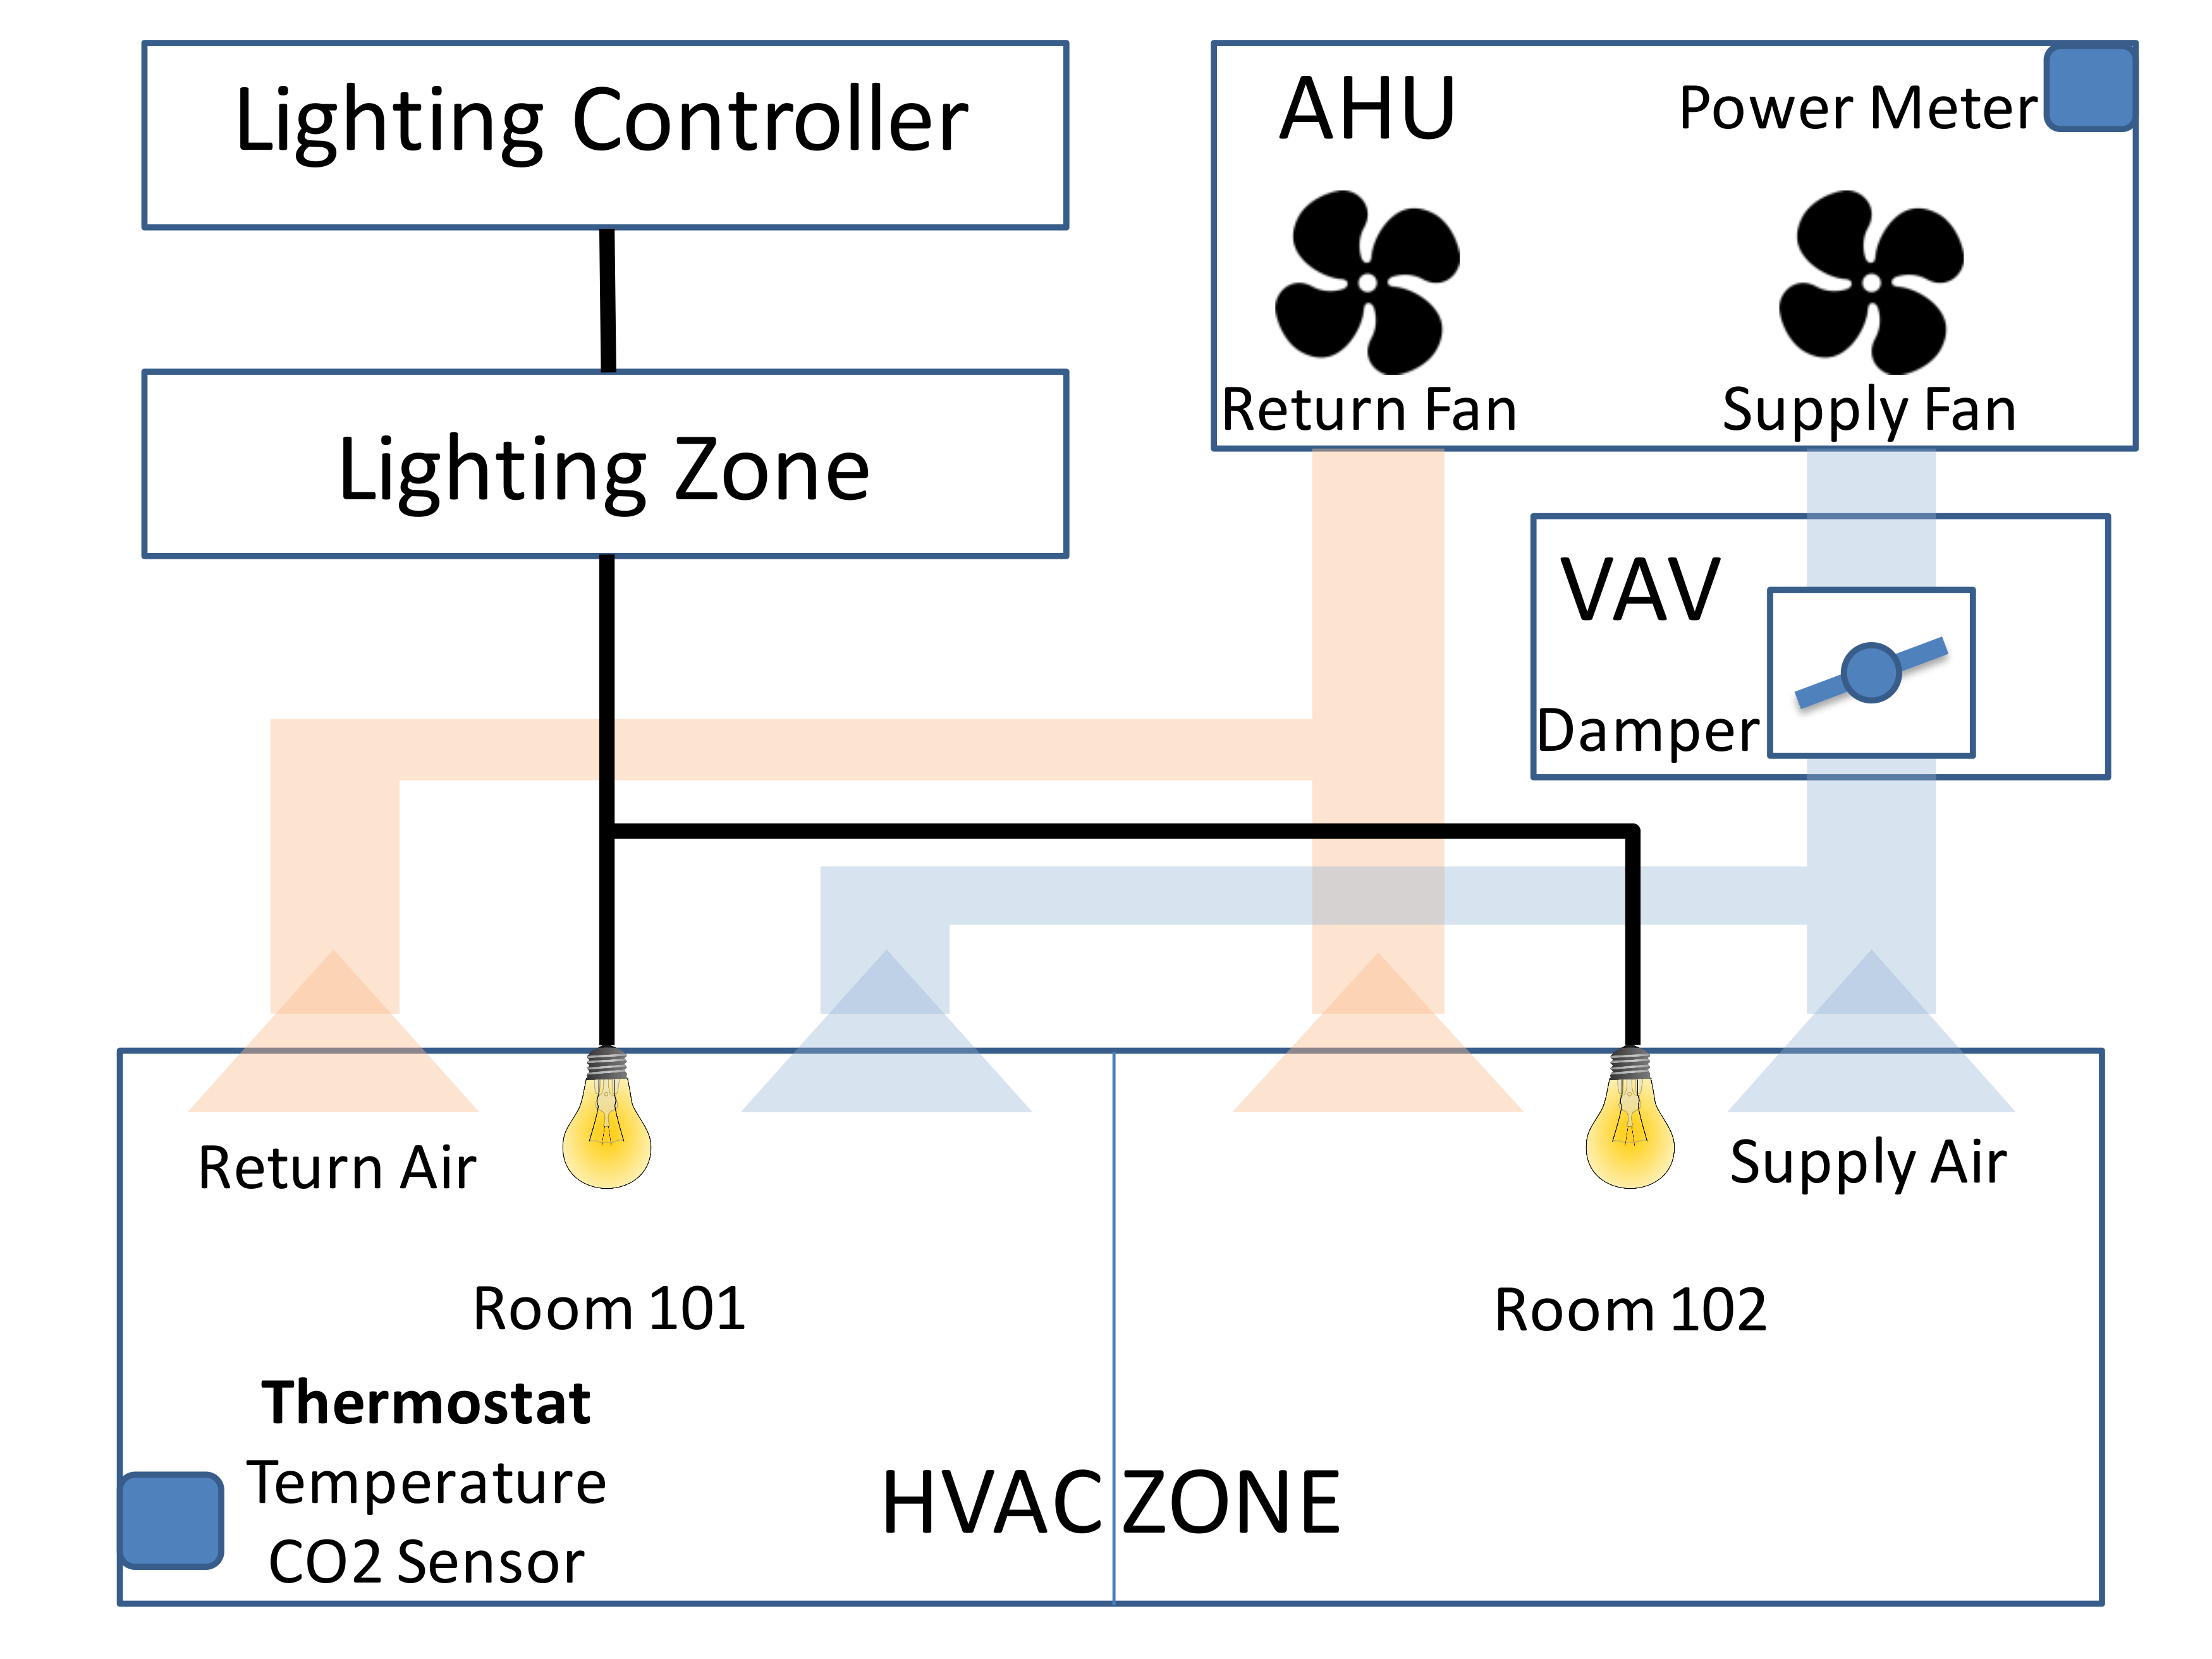
\includegraphics[width=.5\linewidth]{figs/example_building}
\caption{A simple representation of a building's subsystems. Note how a single VAV conditions two separate rooms based on the input from a single thermostat.}
\label{fig:example_building}
\end{figure}

\subsection{Applying the Ising Model}

Our approach is as follows:

\begin{itemize}
\item to decompose a physical space consisting of rooms and hallways into ``microzones''
\item to model the microzones and their connections (be this a door or a window or open air) as nodes and edges in a pairwise undirected graph
\item to use real-world temperature data gathered from an array of wireless sensor motes deployed across the rooms and microzones as data on which we can run parameter estimation to retrieve the edge potentials
\item the edge potentials will indicate the tendency of two neighboring microzones to experience similar changes in temperature, which we can interpret as a measure of the thermal coupling between those two microzones
\end{itemize}

\begin{figure}
\centering
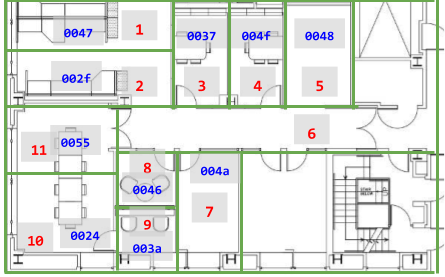
\includegraphics[width=.5\linewidth]{figs/Soda_AMP_microzones}
\caption{Microzones in the south-west corner of Soda Hall's AMP lab. Red numbers are zone labels; blue numbers are sensor labels. Microzones were chosen such that there was a sensor in each zone, with the exception of node 6 which represents the hallway.}
\label{fig:soda_amp_microzones}
\end{figure}


\begin{figure}
\centering
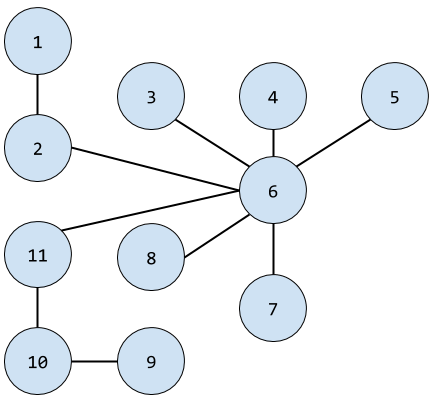
\includegraphics[width=.5\linewidth]{figs/SodaEdgeGraph}
\caption{The undirected graph representing the south-west corner of Soda Hall's AMP lab. Edges reflect physical connections between rooms -- either by door or by open air. We also explore a fully-connected graph with the same set of nodes.}
\label{fig:physical_soda_edges}
\end{figure}


\if 0
Why Buildings?
- buildings use 40% of energy:
    - have lots of sensors, automated control systems
    - these are often incomplete or out of date
    - much manual effort to repair this, or to build up metadata
    - metadata can help buildings be more efficient and comfortable:
        - simultaneous heating/cooling
        - misplaced thermostats (like behind 410 soda screen)
    - want to reason about how buildings behave:
      - building models one approach, but expensive and hard to do and become out of date
      - need another method, one that can be somewhat automated and not require
        immense amounts of domain expertise

Problem Description:
- buildings assume temperature is uniform across an HVAC zone: how true is this really?
    - two complementary questions:
      1. Can we determine the nature of thermal coupling between sub-hvac-zones?
      2. Could we reconstruct the assignment of rooms to hvac zones from this information?
    - We don't address the second, but we explore the first

\fi
